%!TEX root = ./seminarpaper.tex


\chapter{Implementation}

The general idea is that every function gets its own java class inside the \lstinline{functions} folder of the newly created folder structure. For the authors this meant implementing one java class for every statistical distribution function. However, the basic concept is the same for any new function. 

\section{Basic Concept}

First of all, the name of the java class has to follow a certain naming pattern to be recognized as a function. The pattern consists of the following elements:

\begin{itemize}
	\item \lstinline{PD_}
	\item \lstinline{name of the function which will be used to call it inside the interpreter}
	\item \lstinline{.java}
\end{itemize}

The function to compute the normal distribution for example would thus be stored in a file called \lstinline{PD_stat_normal.java}. After creating the file, the next important step is to choose the correct class to extend. For the class to be recognized as a function, it \textbf{must} extend \lstinline{PreDefinedProcedure}, which is basically the template for any function that should later be accessible from within the interpreter. In case of the normal distribution function, the first line of the file should then look like this:

\begin{center}
	\begin{lstlisting}[caption={Class Definition}, language={java}, label=lis:classDefinition]
		public class PD_stat_normal extends PreDefinedProcedure {
	\end{lstlisting}
\end{center}

Some functions may require certain parameters for their execution. These parameters are defined directly after the class definition as variables of the predefined type \lstinline{ParameterDefinition}. They are created by using the \lstinline{createParameter()} method of the base class \lstinline{PreDefinedProcedure}. The only parameter this method takes is a string which determines the name of the variable to be created. The normal distribution function for example requires three parameters, \textit{x}, $\mu$ and $\sigma$. The parameter definitions in the corresponding file would thus look like this:

\begin{center}
	\begin{lstlisting}[caption={Parameter Definition}, language={java}, label=lis:parameterDefinition]
		private final static ParameterDefinition X     = createParameter("x");
		private final static ParameterDefinition MU    = createParameter("mu");
		private final static ParameterDefinition SIGMA = createParameter("sigma");
	\end{lstlisting}
\end{center}

To finish up the formal definition of a function, a default constructor is needed which is then used to create an instance of the class as an instance of \lstinline{PreDefinedProcedure} with the name \lstinline{DEFINITION}. Shown below is the case of the normal distribution function:

\begin{center}
	\begin{lstlisting}[caption={Constructor and Function Definition}, language={java}, label=lis:constructor]
		/** Definition of the PreDefinedProcedure 'stat_normal' */
		public final static PreDefinedProcedure DEFINITION = new PD_stat_normal();

		private PD_stat_normal() {
			super();
			addParameter(X);
			addParameter(MU);
			addParameter(SIGMA);
		}
	\end{lstlisting}
\end{center}

Up to this point, everything that was done can basically be done for any new function by just changing the name and the required parameters. The thing that sets every function apart is the \lstinline{execute} method that needs to be overridden when extending \lstinline{PreDefinedProcedure}. This method is called when the function gets called as a \setlx\ function from within the interpreter. It takes the parameters that were defined for the function, performs some computation with these parameters and returns the result which is then shown in the interpreter.

\section{Computation}

Any parameter that a function gets called with is given to the \lstinline{execute} method within an array called \lstinline{args}. From this array every parameter can be retreived by calling \lstinline{args.get(NAME)} with \lstinline{NAME} being one of the names of the \lstinline{ParameterDefinition} variables that were defined for the function. Since the \lstinline{execute} 
method bears almost no common concepts between different kinds of functions but shows high similarities across all statistical distribution functions that were implemented by the authors, the normal distribution function will be used as an example in this chapter to show the work of the authors and provide a basic understanding of what the \lstinline{execute} method is supposed to do and how it could be implemented for new functions. The purpose of this function is to compute the propability density at some point \textit{x} with given parameters $\mu$ and $\sigma$. To start, the method definition and the retrieval of all parameters for the normal distribution function can be seen below:

\begin{center}
	\begin{lstlisting}[caption={Execute method and parameter retrieval}, language={java}, label=lis:parameterRetrieval]
		/** Definition of the PreDefinedProcedure 'stat_normal' */
		@Override
		public Value execute(State state, HashMap<ParameterDefinition, Value> args) throws SetlException {
		
        final Value x     = args.get(X);
        final Value mu    = args.get(MU);
        final Value sigma = args.get(SIGMA);
	\end{lstlisting}
\end{center}

 Note that at this point of execution, every parameter is of the abstract type \lstinline{Value}. One characteristic of statistical distribution functions is that in many cases the parameters have to fit certain criteria for the function to execute correctly. The most important one, which is applicable to all distribution functions, is that only numbers are allowed as parameters. Special to the normal distribution function is the requirement that the parameter $\sigma$ is greater than zero. To check if the parameters that the function was called with fit this criteria, a utility class called \lstinline{Checker} was implemented. This class is stored in the folder \lstinline{utility}, which was created on the level of the \lstinline{functions} folder and contains many different \lstinline{check} methods for any criteria that a distribution function may demand. Shown below are the implementations of the methods \lstinline{checkIfNumber} and \lstinline{checkIfNumberAndGreaterZero}:
 
 \newpage
 \begin{center}
	\begin{lstlisting}[caption={Checker methods}, language={java}, label=lis:checkerMethods]
		/** Checks if given values are numbers and if not, throws an exception */
		public static boolean checkIfNumber(State state, Value... values) throws IncompatibleTypeException {
			for (Value value : values) {
				if (! (value.isRational() == SetlBoolean.TRUE || value.isDouble() == SetlBoolean.TRUE)) {
					throw new IncompatibleTypeException(
						"Input-argument '" + value.toString(state) + "' is not a number."
					);
				}
			}
			return true;
		}

		/** Checks if given values are numbers and greater zero and if not, throws an exception */
		public static boolean checkIfNumberAndGreaterZero(State state, Value... values) throws SetlException {
			for (Value value : values) {
				if (! (value.isRational() == SetlBoolean.TRUE || value.isDouble() == SetlBoolean.TRUE)) {
					throw new IncompatibleTypeException(
							"Input-argument '" + value.toString(state) + "' is not a number."
					);
				}
				if (! (value.toJDoubleValue(state) > 0)) {
					throw new IncompatibleTypeException(
						"Input-argument '" + value.toString(state) + "' is not greater than zero."
					);
				}
			}
			return true;
		}
	\end{lstlisting}
\end{center}

If every given parameter was checked and none of the \lstinline{checker} methods threw an exception, the actual computation of the statistical distribution can begin. To do this computation, the authors have chosen the \href{http://commons.apache.org/proper/commons-math/userguide/distribution.html}{Apache Commons Math} library due to a vast number of statistical distributions being supported. To perform calculations with a certain statistical distribution, an object of that distribution has to be created via its constructor using the function-specific parameters, which would be $\mu$ and $\sigma$ in case of the normal distribution. On this object the methods \lstinline{density(x)} and \lstinline{cumulativePropability(x)} can be called to compute the propability density or the cumulative propability for some value \textit{x} respectively. Putting it all together, the computation of the propability density for normal distributions looks like this:

\begin{center}
	\begin{lstlisting}[caption={Normal Distribution propability density computation}, language={java}, label=lis:densityComputation]
		NormalDistribution nd = new NormalDistribution(mu.toJDoubleValue(state), sigma.toJDoubleValue(state));
        return SetlDouble.valueOf(nd.density(x.toJDoubleValue(state)));
	\end{lstlisting}
\end{center}

The method \lstinline{toJDoubleValue(state)} that can be seen in the first line of the code above, converts the parameter it is used on from the abstract type \lstinline{Value} into a primitive \lstinline{double} value. This is done because the library can of course only calculate using primitive data types. On the other hand this means that before the result can be returned, it has to be converted back into a data type that the \setlx\ interpreter understands, in this case \lstinline{SetlDouble}. This finally is what is shown in the interpreter as the result of the function.

\section{Graphical Output}

While working on the first few distribution functions, the authors noticed that it would be nice to have some sort of graphical representation for the output of these functions. Fortunately, an addon for \setlx\ that deals with graphical output already exists, so it was decided to use this to implement an additional function for every statistical distribution function that creates a graphical representation of the computed result. The main difference of these functions to their the non-graphical counterpart is the absence of a concrete \textit{x} - value. The idea was to show the graph of a function in a certain interval for some provided parameters. The interval of the graph is also adjustable when calling the function in \setlx. To compute this graph, the function loops over all numbers between the lower end and the upper end of the interval in a step size that can also be adjusted. In every iteration, a result is computed for the current value. The value and the result for this value are then added to a list as \textit{x} and \textit{y} coordinates which is then used to create the graph. To avoid having the user to provide the interval and the step size every time when calling the function, these parameters are only optional parameters and are defined with a default value for every function.

\begin{center}
	\begin{lstlisting}[caption={Optional Parameters for Bounds and Interval}, language={java}, label=lis:boundsInterval]
		private final static ParameterDefinition MU          = createParameter("mu");
		private final static ParameterDefinition SIGMA       = createParameter("sigma");
		private final static ParameterDefinition CANVAS      = createParameter("canvas");
		private final static ParameterDefinition COLOR       = createOptionalParameter("color", new SetlString("DEFAULT_COLOR"));
		private final static ParameterDefinition LOWER_BOUND = createOptionalParameter("lowerBound", Defaults.createSetlDoubleValue(-5.0));
		private final static ParameterDefinition INTERVAL    = createOptionalParameter("interval", Defaults.getDefaultPlotInterval());
		private final static ParameterDefinition UPPER_BOUND = createOptionalParameter("upperBound", Defaults.createSetlDoubleValue(5.0));
	\end{lstlisting}
\end{center}

Listing \ref{lis:boundsInterval} shows the parameter definitions for the function \lstinline{stat_normal_plot}, which demonstrate how optional parameters are defined using the \lstinline{createOptionalParameter()} - method. Important to note here is the parameter canvas: This is part of the \lstinline{plot} - addon and represents the surface any graphical output is drawn on. The color of the output graph may be adjusted by providing a color
parameter of the form [R,G,B] (an array with three values - red, green and blue). For example, calling \lstinline{stat_normal_plot(canvas, mu, sigma, [255, 0, 0])} would produce a red graph. 
\begin{center}
	\begin{lstlisting}[caption={Computation of propability density graph for Normal Distributions}, language={java}, label=lis:densityGraph]
		NormalDistribution nd = new NormalDistribution(mu.toJDoubleValue(state), sigma.toJDoubleValue(state));

        /** The valueList is the list of every pair of coordinates [x,y] that the graph consists of.
         *  It is filled by iteratively increasing the variable 'counter' (x), and calculating the density for every new value of 'counter' (y).
         */
        List<List<Double>> valueList = new ArrayList<>();
        for (double counter = lowerBound.toJDoubleValue(state); counter < upperBound.toJDoubleValue(state); counter += interval.toJDoubleValue(state)) {
            valueList.add(new ArrayList<Double>(Arrays.asList(counter, nd.density(counter))));
        }

        return ConnectJFreeChart.getInstance().addListGraph((Canvas) canvas, valueList, "Probability Density Function (mean: " + mu.toString() + ", standard deviation: " + sigma.toString(), Defaults.DEFAULT_COLOR_SCHEME, false);
	\end{lstlisting}
\end{center}

Shown in listing \ref{lis:densityGraph} is the loop that computes the list of coordinates for the graph, using the same objects and methods that the non-graphical version of the normal distribution function. In the last line, the \lstinline{plot} - addon is then used to draw the graph on the given canvas and create a graphical output that is shown to the user. An example for the case of the normal distribution is shown below:

\begin{figure}[h]
    \centering
    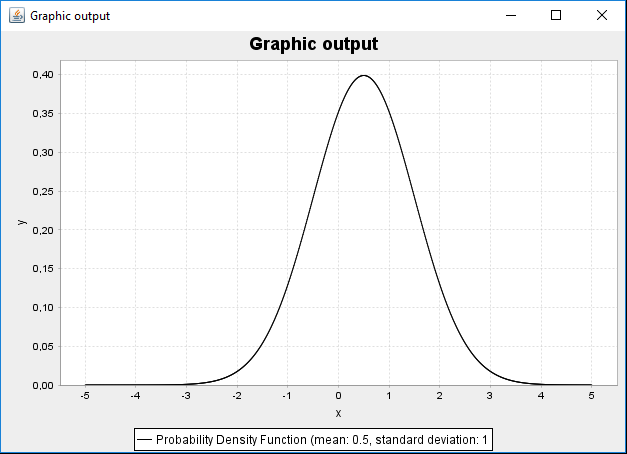
\includegraphics[width=1\textwidth]{Figures/implemented_functions/normal_pdf}~\\
    \caption{Normal Distribution Plot}
    \label{fig:normalDistPlot}
\end{figure}